%%=============================================================================
%% Methodologie
%%=============================================================================

\chapter{\IfLanguageName{dutch}{Methodologie}{Methodology}}
\label{ch:methodologie}

%% TODO: Hoe ben je te werk gegaan? Verdeel je onderzoek in grote fasen, en
%% licht in elke fase toe welke stappen je gevolgd hebt. Verantwoord waarom je
%% op deze manier te werk gegaan bent. Je moet kunnen aantonen dat je de best
%% mogelijke manier toegepast hebt om een antwoord te vinden op de
%% onderzoeksvraag.

In het vorige hoofdstuk werd de eerste deelonderzoeksvraag beantwoord, namelijk wat de voor- en nadelen van een cross-platform framework zijn. In dit hoofstuk wordt er stapgewijs een antwoord gegeven op de deelonderzoeksvragen om zo tot een antwoord te komen op de hoofdonderzoeksvraag van deze studie. Alvorens een vergelijking kan gemaakt worden tussen enkele frameworks en dus de volgende deelonderzoeksvragen beantwoord kunnen worden moet er bepaald worden welke frameworks voldoen aan de eisen die gesteld worden door het team. Deze worden onderverdeeld in functionele en niet-functionele eisen en zijn te vinden in sectie \ref{sec:eisen-framework}. In sectie \ref{sec:selectieFrameworks} worden de populairste cross-platform frameworks op het moment van schrijven van deze studie opgesomd en kort besproken. Vervolgens worden deze in sectie \ref{sec:aftoetsenEisen} afgetoetst tegenover de gestelde eisen. Eens de finale lijst voor de vergelijking is opgesteld worden de geselecteerde frameworks met elkaar vergeleken in sectie \ref{sec:vglEigenschappen}.

\section{Eisen framework}
\label{sec:eisen-framework}

Om een lijst van frameworks die zinvolzijn om te vergelijken met elkaar moeten de frameworks voldoen aan enkele vooropgestelde eisen. In deze sectie worden deze eisen besproken, met een opslitsing tussen functionele en niet-functionele eisen.

\subsection{Functionele eisen}
\label{subsec:functioneleEisen}

De functionele eisen die gesteld worden aan het framework zijn:

\begin{enumerate}
    \item Apps zien er native uit
    \item Apps hebben dezelfde performantie als native apps
    \item Apps kunnen offline gebruikt worden (indien er functies zijn die geen netwerkverbinding nodig hebben)
    \item Er kan gebruik gemaakt worden van de native API's (native functionaliteiten)
\end{enumerate}

\subsubsection{Motivatie functionele eisen}
\label{subsubsec:MotivatieFunctioneleEisen}

Voor gebruikers van een applicatie is het zeer belangrijk dat de gebruikersinterface van een applicatie overeenkomt met wat ze gewoon zijn van andere applicaties. Dit houdt in dat ze op dezelfde manier moeten kunnen navigeren, knoppen en symbolen moeten er hetzelfde kunnen uitzien, widgets moeten native aanvoelen en ga zo maar door. Dit alles zorgt ervoor dat het gebruiksgemak van de applicatie gevoelig beter wordt. Niet enkel hoe applicaties er uit zien is belangrijk voor gebruikers, ook de performantie ervan is een zeer belangrijk punt. Niemand heeft graag een app die hapert of ellendig lang duurt om te laden. 

Verder is het ook belangrijk dat een app die beschikt over functionaliteit waarvoor geen netwerkconnectie vereist is ook offline gebruikt kan worden. De applicatie moet dus op het apparaat zelf geïnstalleerd kunnen worden en er moet lokale data bijgehouden kunnen worden. Een laatste eis is er één vanuit het oogpunt van de ontwikkelaars: om de gebruikers een native ervaring te kunnen aanbieden heeft de ontwikkelaar toegang nodig tot de native API's. Door deze eis te stellen wordt er verzekerd dat het framework toelaat om alle aanwezige hardwarefunctionaliteiten van een systeem te gaan benutten.

\subsection{Niet-functionele eisen}
\label{subsec:nietFunctioneleEisen}

Net als bij de functionele eisen volgt ook hier eerst een opsomming, waarna de motivatie voor het stellen van deze eisen gegeven wordt. De niet-functionele eisen aan het framework zijn:

\begin{enumerate}
    \item Reeds aanwezige kennis van de programmeertaal binnen het team
    \item Grote en actieve community (en dus een populair framework)
    \item Voldoende documentatie beschikbaar
    \item Regelmatige updates van het framework
    \item Recente laatste stabiele versie (geen verouderd framework)
    \item Toekomstige ondersteuning gegarandeerd    
\end{enumerate}

\subsubsection{Motivatie niet-functionele eisen}
\label{subsubsec:MotivatieNietFuntioneleEisen}

Om vlot aan de slag te kunnen met het framework is het een grote meerwaarde als de programmeertaal reeds gekend is binnen het team. Op deze manier kan het team zich onmiddellijk focussen op de specifieke eigenschappen van het framework, in plaats van eerst de syntax van de taal te moeten leren. Eens de ontwikkelaars effectief een app aan het schrijven zijn is de kans zeer groot dat ze zaken tegen komen die ze niet direct zelf kunnen oplossen. In deze situaties is het noodzakelijk om te kunnen terugvallen op de officiële documentatie van het framework en op een community die klaar staat om te helpen (denk maar aan issues op GitHub, vragen op Stackoverflow, ...). Verder is een actieve community een goede indicatie dat het framework 'leeft' en dus ook updates zal ontvangen. Regelmatige updates zijn noodzakelijk voor elk softwareprogramma. Er zijn voortdurend nieuwe ontwikkelingen en nieuwe bedreigingen. Om moderne en veilige applicaties te schrijven (en deze zo te houden) is een framework met regelmatige updates dus onontbeerlijk. Vanuit datzelfde oogpunt is ook een recente stabiele versie een belangrijke eis. Tot slot is het doel van deze studie om een aanbeveling te kunnen doen van een framework dat geschikt is om de komende jaren mee aan de slag te gaan. Het is dus zeer belangrijk dat toekomstige ondersteuning gegarandeerd is. Hiermee wordt bedoeld dat er updates zullen uitgebracht blijven worden, met nieuwe functionaliteiten en de laatste nieuwe beveiligingsmethodes.

\section{Selectie frameworks}
\label{sec:selectieFrameworks}

In de vorige sectie werden de eisen gedefinieerd waaraan de frameworks binnen deze studie moeten voldoen. In deze sectie worden alle populaire cross-platform frameworks opgesomd en wordt er per kort framework een korte uitleg gegeven over de achtergrond van het framework.

\subsection{Lijst van populairste cross-platform frameworks}

Om tot een lijst van de populairste frameworks te komen werd gekeken naar de resultaten van een wereldwijde ondervraging door JetBrains \autocite{Liu2020}. Met 19696 deelnemers aan deze ondervraging is dit een zeer goede weergave van de populariteit van de verschillende frameworks onder ontwikkelaars.

In figuur \ref{fig:frameworkPopularity} zijn de resultaten van deze ondervraging te zien. Uit deze figuur blijkt dat er enkele zeer populaire frameworks zijn, waarvan React Native en Flutter de populairste zijn. Een interessante opmerking is dat de populariteit van Flutter sterk gestegen is (+9\%) in 2020 in vergelijking met 2019, waar die van React Native hetzelfde gebleven is (42\%). Anderzijds is de populariteit van enkele andere frameworks sterk gedaald: Cordova (-11\%), Ionic (-10\%) en Xamarin (-12\%) zijn een heel pak gebruikers kwijt geraakt. Tot slot zijn helemaal rechts enkele frameworks te zien die in 2019 door geen enkele van de ondervraagden gebruikt werden maar in 2020 wel een bepaald (weliswaar laag) percentage gebruikers weten te overtuigen. Zo duikt bijvoorbeeld Kotlin Multiplatform op in de ondervraging, met 2\% van de ondervraagden die aangeven dit te gebruiken. Ook Kivy en Corona duiken op in de resultaten van de ondervraging in 2020 met elk 1\% van de ondervraagden die aangeeft er gebruik van te maken.

Alle frameworks die aan bod komen in deze ondervraging zullen in de volgende sectie kort besproken worden en vervolgens afgetoetst worden tegen de gestelde eisen (behalve Apache Flex en Dojo, gezien de reeds beperkte populariteit in 2019 en de daling in populariteit in 2020). Het is namelijk niet automatisch zo dat het (op dit moment) populairste framework ook meteen de beste keuze is voor de komende jaren.

Verder wordt ook .NET MAUI besproken in deze studie. Dit is een cross-platform framework dat op 19/5/2020 uitgebracht werd door Microsoft. Omdat delaware een partner is van Microsoft en het team reeds werkt met .NET voor de ontwikkeling van de backend van de applicaties is het zeker een interessant framework om mee te nemen in de vergelijking. Recentere frameworks hebben namelijk het voordeel dat ze enkele tekortkomingen van eerdere frameworks makkelijker kunnen opvangen en kunnen dus zeker ook een goede keuze zijn voor de toekomst.

\begin{figure}
    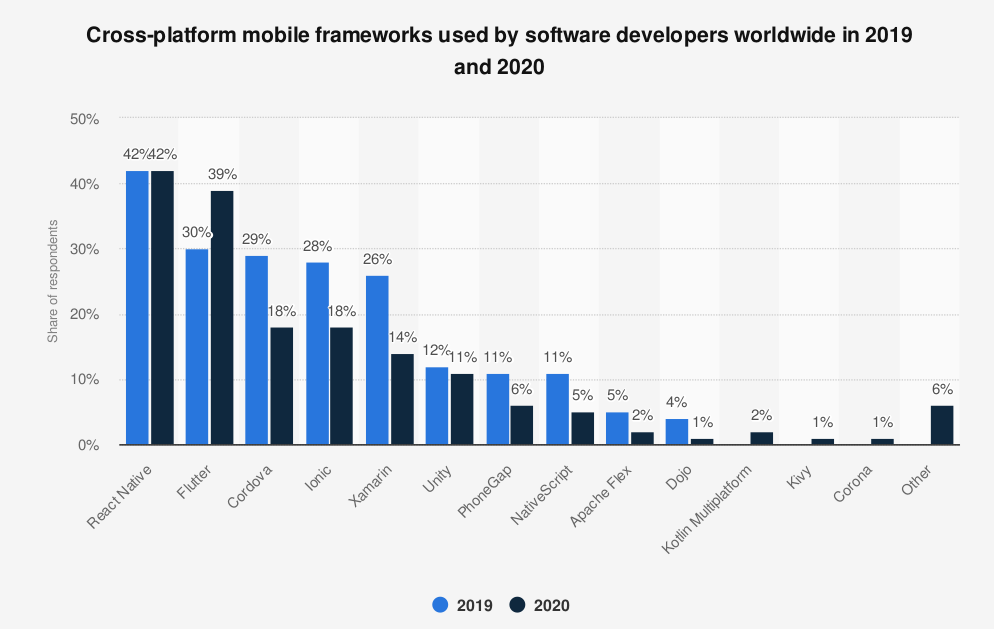
\includegraphics[width=\linewidth]{PopularFrameworksGraph.png}
    \caption{Resultaten van de populariteitsondervraging van cross-platform frameworks door JetBrains}
    \label{fig:frameworkPopularity}
\end{figure}

\subsection{Achtergrond frameworks}
\label{subsec:achtergrondFrameworks}

Alle frameworks die in de ondervraging van JetBrains aan bod komen worden in de volgende paragrafen kort besproken, met uitzondering van Apache Flex en Dojo. Deze beide frameworks hadden reeds een beperkte populariteit en die is dan nog eens sterk gedaald op een jaar tijd ook. Dit is een teken dat het framework niet zo goed is als andere opties en het heeft dus geen nut van hier aandacht aan te besteden.

\subsubsection{React Native}
\label{subsubsec:ReactNative}

React Native (2015) is een open source cross-platform framework dat ontwikkeld is en onderhouden wordt door Facebook \autocite. Zoals de naam al doet vermoeden steunt dit framework op React (een Javascript library, ook ontwikkeld door Facebook). React is speciaal ontwikkeld om gebruikersinterfaces te maken, maar waar React zelf zich richt op webbrowsers focust React Native zich op mobiele platformen. Met behulp van React Native kunnen applicaties geschreven worden die er helemaal native uitzien en dit in een taal die reeds heel erg gekend is onder ontwikkelaars \autocite{Eisenman2015}.

\subsubsection{Flutter}
\label{subsubsec:Flutter}

Flutter is een software development kit (SDK) ontwikkeld door Google in 2017. Het is een 'UI toolkit' om native gecompileerde apps te maken die er mooi uitzien met een enkele broncode \autocite{Google2020}. Net zoals React Native is ook Flutter volledig open source. Het kan rekenen op een grote community en voortdurende verdere ontwikkeling. De laatste stabiele versie van Flutter werd uitgebracht door Google op 6/5/2020. Het is dus een zeer recente update waardoor de SDK kan rekenen op de laatste nieuwe ontwikkelingen op het vlak van cross platform development. Flutter apps worden geschreven in Dart, een object georiënteerde programmeertaal gebaseerd op klassen en ontwikkeld door Google. Het grote voordeel van Dart is dat het gecompileerd kan worden naar Javascript maar ook rechtstreeks naar native code, wat een groot voordeel oplevert op het vlak van prestaties.

\subsubsection{Cordova}
\label{subsubsec:Cordova}

Cordova is een framework dat ontwikkeld is door Adobe en bestaat al sinds 2011. Het werd in 2013 overgedragen aan Apache om het open source karakter van het framework te kunnen garanderen . Het framework kan gebruikt worden voor het ontwikkelen van cross-platform mobiele applicaties. De talen die gebruikt worden zijn HTML5, CSS3 en Javascript \autocite{Apache2020}. Dit zijn de standaard talen voor de ontwikkeling van webapplicaties, een ontwikkelaar moet dus geen nieuwe taal leren om met Cordova aan de slag te gaan. Applicaties worden uitgevoerd binnen specifieke wrappers per platform en maken gebruik van de native API's om de specifieke hardware componenten van een systeem te gebruiken.

\subsubsection{Ionic}
\label{subsubsec:Ionic}

Ionic is een UI toolkit voor het maken van mobiele webapplicaties. Het is ontwikkeld door Ionic zelf en is een open source project. Ionic bestaat uit drie lagen. De basis is Apache Cordova: het is dus een distributie van Cordova en voegt hier extra eigenschappen aan toe. Bovenop Cordova is er een frontend framework geplaats voor het ontwikkelen van de gebruikersinterface. In de eerste versies van Ionic was dit Angular, maar sinds versie 4 is de gebruiker zelf vrij om te kiezen. Er is ondersteuning aanwezig voor Angular, React, Vue.js en web componenten \autocite{Schiemann2019}. Ionic geeft de ontwikkelaar dus zelf de keuze met welk frontend framework gewerkt wordt. De laatste laag tot slot is het Ionic framework zelf: de visuele weergave van het framework en een set van componenten die het mogelijk maken om op een eenvoudige manier de gebruikersinterface te beschrijven.

\subsubsection{Xamarin}
\label{subsubsec:Xamarin}

Xamarin is een uitbreiding van het .NET platform van Windows. Het levert een framework dat toegang geeft tot de native eigenschappen van een platform, libraries om de native API's te kunnen gebruiken en een eigen markup taal (XAML) om de gebruikersinterface te beschrijven \autocite{Microsoft2020}. Het grote voordeel van het feit dat Xamarin .NET uitbreid is dat alle mogelijkheden en ondersteuning van .NET ook beschikbaar is voor Xamarin. Ontwikkelaars die reeds gewoon zijn om met .NET te werken kunnen dus onmiddellijk aan de slag met het ontwikkelen van mobiele applicaties met dit framework.

\subsubsection{Unity}
\label{subsubsec:Unity}

Unity is een cross-platform framework dat zich richt op het ontwikkelen van games voor mobiele apparaten. Het is uitermate geschikt voor het creëren van 3D content en complexe graphics. 

\subsubsection{PhoneGap}
\label{subsubsec:PhoneGap}

PhoneGap is, net als Ionic, een distributie van Apache Cordova. Het steunt op dezelfde principes maar heeft een eigen gebruikersinterface en extra services. Het is in handen van Adobe (de originele ontwikkelaar van Cordova). Hoewel het in se dus hetzelfde is als Cordova, zijn er bij PhoneGap enkele functionaliteiten extra van Adobe (zoals PhoneGap Build Service, een service die ontwikkelaars toelaat om apps te builden in de cloud).

\subsubsection{NativeScript} 
\label{subsubsec:NativeScript}

NativeScript is een open source framework voor het bouwen van mobiele applicaties die native aanvoelen. Net als bij Ionic kan er gebruik gemaakt worden van verschillende frontend frameworks (Angular en Vue.js) of de ontwikkelaar kan aan de slag met JavaScript of TypeScript \autocite{NativeScript2020}. Het grootste voordeel van NativeScript is dat het rechtstreekse toegang geeft tot de native API's. De ontwikkelaar moet dus niet wachten tot iemand een brug geschreven heeft om nieuwe eigenschappen te gebruiken. Van zodra nieuwe eigenschappen beschikbaar zijn van een platform kan de ontwikkelaar deze gebruiken. NativeScript is dus geen wrapper rond een WebView, in tegenstelling tot vele andere cross-platform frameworks \autocite{Anderson2016}.

\subsubsection{Kotlin Multiplatform}
\label{subsubsec:Kotlin}

Kotlin is een open source SDK die de ontwikkelaar toelaat om cross-platform applicaties te schrijven en uitgebracht is door JetBrains. Door het feit dat dit een SDK is kan de ontwikkelaar delen van de applicatie in Kotlin schrijven, zonder dat de gehele applicatie opnieuw geschreven hoeft te worden (zoals wel het geval is bij een framework). Verder laat Kotlin Multiplatform ook toe om toch platform specifieke code te schrijven indien er zaken zijn die niet cross-platform opgelost kunnen worden. Door deze mogelijkheid kan de ontwikkelaar ook onmiddellijk inspringen op nieuwe eigenschappen van een platform: van zodra een eigenschap beschikbaar is kan deze ook gebruikt worden in de applicatie \autocite{JetBrains2020}. De mogelijkheid voor het schrijven van cross-platform applicaties met Kotlin is wel nog een experimentele functionaliteit, die beschikbaar is sinds versie 1.3 \autocite{Belov2018}.


\subsubsection{Kivy}
\label{subsubsec:Kivy}

Kivy is een open source grafische gebruikersinterface library die het mogelijk maakt om met Python cross-platform mobiele applicaties te schrijven \autocite{Vasilkov2015}. Het stelt de ontwikkelaar in staat om innovatieve gebruikersinterfaces te maken, zoals multi-touch apps. Het is in staat om zware grafische gebruikersinterfaces te tonen en dus ook geschikt voor het ontwikkelen van mobiele games \autocite{Kivy2020}. De eerste release van de library was op 1/2/2011. Het is dus een library die al een tijdje mee gaat en dus geen last meer heeft van kinderziektes.

\subsubsection{Corona}
\label{subsubsec:Corona}

Corona is een cross-platform framework dat ideaal is voor het snelle ontwikkelen van mobiele applicaties en games. Het is gebaseerd op Lua, een open source scripting taal. Er zijn vele plugins beschikbaar en er is toegang tot de native API's indien er geen plugin beschikbaar is voor een bepaalde eigenschap. Het framework beschikt over een simulator die de ontwikkelaar toelaat om aanpassingen direct te kunnen zien \autocite{Coronalabs2020}. Een nadeel is wel dat het bedrijf achter Corona niet meer bestaat sinds 1/5/2020. De software gaat verder als een open source project, maar het toekomstige bestaan en updates zijn dus niet langer gegarandeerd \autocite{Shcherban2020}.

\subsubsection{.NET MAUI}
\label{subsubsec:.NETMAUI}

.NET MAUI (Multi-platform App UI) is een cross-platform framework dat op 19/5/2020 uitgebracht werd door Microsoft \autocite{Hunter2020}. Op de datum van schrijven van deze studie is dit dus nog een zeer recent framework, dat nog niet veel bekendheid en gebruikers heeft. Het is een verdere evolutie van Xamarin, een ander cross-platform framework van Microsoft. Microsoft heeft als doel om met .NET MAUI een framework aan te bieden dat niet enkel dient om applicaties te schrijven voor smartphones, maar ook voor computers, tablets en andere apparaten waarop applicaties geïnstalleerd kunnen worden. Zoals de naam al doet vermoeden steunt het framework op .NET. Ontwikkelaars die reeds ervaring hebben met dit framework (en C\#, de taal die gebruikt wordt bij .NET) hoeven dus geen nieuwe taal of nieuw framework te leren. De effectieve release van een stabiele versie van het framework is gepland samen met het uitbrengen van .NET 6 in november 2021. Ondertussen kunnen ontwikkelaars wel previews verwachten van het framework, waarvan de eerste zal uitkomen op het einde van 2020 \autocite{Suarez2020}. Het is de bedoeling van Microsoft dat .NET MAUI de opvolger van Xamarin wordt. Xamarin zal wel nog onderhouden worden, maar alle nieuwe ontwikkelingen zullen in .NET MAUI komen.

\section{Aftoetsen eisen framework}
\label{sec:aftoetsenEisen}

De populairste cross-platform frameworks van de voorbije twee jaar werden besproken in de vorige sectie. In deze sectie worden de verschillende frameworks afgetoetst tegen de gestelde eisen om op deze manier tot een finale lijst van frameworks te komen die in de rest van de studie met elkaar vergeleken zullen worden.

\subsection{Functionele eisen}
\label{subsec:aftoetstenFunctioneleEisen}

De funtionele eisen die gesteld worden aan het framework zijn te vinden in sectie \ref{subsec:functioneleEisen}. Al de hiervoor vooropgestelde frameworks voldoen aan alle functionele eisen die gesteld worden aan het framework. Deze worden dus niet afzonderlijk opgesomd. Om tot een verkleinde lijst van frameworks te komen om te kunnen gaan vergelijken moet er dus gekeken worden naar de niet-functionele eisen.

\subsection{Niet-functionele eisen}
\label{subsec:aftoetsenNietFunctioneleEisen}

De niet-functionele eisen voor het framework zijn te vinden in sectie \ref{subsec:nietFunctioneleEisen}. In tabel \ref{tab:nietFunctioneleEisen} is een overzicht van de resultaten van de verschillende frameworks raadpleegbaar. In de daaropvolgende secties wordt uitleg gegeven bij de frameworks die niet voldoen aan de gestelde niet-functionele eisen.

\begin{table}
    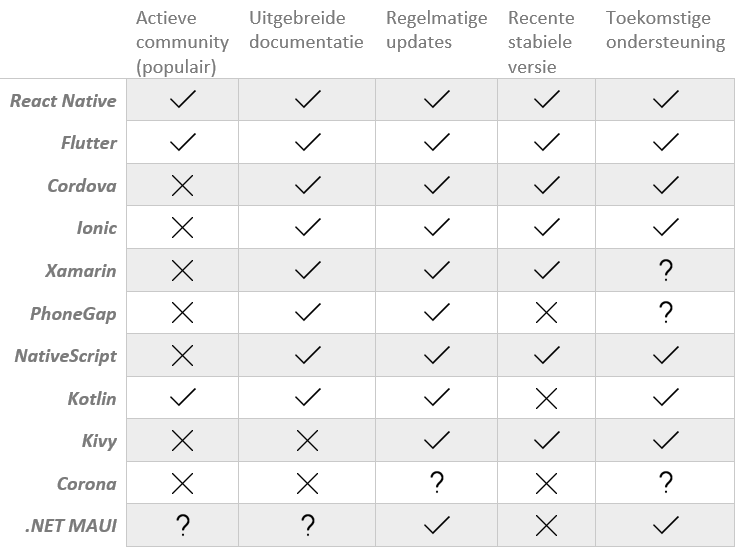
\includegraphics[width=\linewidth]{TabelNietFunctioneleEisen.png}
    \caption{Overzicht aftoetsing niet functionele eisen}
    \label{tab:nietFunctioneleEisen}
\end{table}

\subsubsection{Cordova}
\label{subsubsec:CordovaEisen}

Zoals in tabel \ref{tab:nietFunctioneleEisen} te zien is voldoet Cordova aan alle niet-functionele eisen, behalve aan de populariteitseis. In figuur \ref{fig:frameworkPopularity} is te zien dat de populariteit van het framework sterk gedaald is. Aangezien het framework  de komende jaren gebruikt zal worden is het ook belangrijk dat het framework populair blijft. Een hoge populariteit geeft namelijk meer opties om te gaan gebruiken (denk aan libraries, oplossingen voor specifieke problemen, ...) en is een goede indicatie of het framework zich kan weren tegen andere frameworks. Cordova verliest vele gebruikers aan andere frameworks, waaruit afgeleid kan worden dat andere frameworks een betere optie zijn om te gebruiken.

\subsubsection{Ionic}
\label{subsubsec:IonicEisen}

Aangezien Ionic een distributie is van Cordova en in figuur \ref{fig:frameworkPopularity} te zien is dat ook de populariteit van dit framework sterk gedaald is kan dezelfde conclusie getrokken worden als bij Cordova.

\subsubsection{Xamarin}
\label{subsubsec:XamarinEisen}

In figuur \ref{fig:frameworkPopularity} is een vraagteken te zien bij de toekomstige ondersteuning van Xamarin. Dit komt doordat Microsoft in mei 2020 een nieuw cross-platform framework heeft uitgebracht (.NET MAUI). Microsoft heeft aangekondigd dat Xamarin wel nog onderhouden zal worden maar dat alle nieuwe eigenschappen in .NET MAUI zullen verschijnen en niet langer in Xamarin. Het nieuwe framework is dus eigenlijk de opvolger van Xamarin, waardoor Xamarin geen goede keuze is om de komende jaren op in te zetten.

\subsubsection{NativeScript}
\label{subsubsec:NativeScriptEisen}

NativeScript is een framework dat net als Cordova en Ionic moet inboeten aan populariteit ten opzichte van andere frameworks. Ook hier kan dus dezelfde conclusie getrokken worden dat dit geen goede keuze is om de komende jaren op in te zetten.

\subsubsection{Kotlin}
\label{subsubsec:KotlinEisen}

Kotlin is een framework dat oorspronkelijk gemaakt is voor het ontwikkelen van Android applicaties. Sinds release 1.3 is er ook de mogelijkheid om cross-platform applicaties te schrijven. Deze functionaliteit is echter nog experimenteel, er is dus nog geen stabiele versie van het framework waar cross-platform ontwikkeling een vast deel van uitmaakt. Voor het ontwikkelen van applicaties voor bedrijven in de komende jaren is het absoluut noodzakelijk dat er gerekend kan worden op een stabiele versie van het framework, zodat alle onderteuning die nodig is ook effectief gegarandeerd kan worden. Kotlin is dus met andere woorden op dit moment geen goede optie, al toont het wel zeer veel potentieel.

\subsubsection{Kivy}
\label{subsubsec:KivyEisen}

Kivy is een library die al een hele tijd bestaat, en toch weet deze slechts een zeer klein deel van de ontwikkelaars te overtuigen om het te gebruiken. Verder is ook de documentatie eerder beperkt. Het is dus geen goede optie om de komende jaren hier op in te zetten.

\subsubsection{Corona}
\label{subsubsec:CoronaEisen}

Het grootste probleem van Corona is dat het bedrijf achter het framework niet langer bestaat. Er is dus geen gegarandeerde support in de toekomst, er zijn geen recente stabiele versies beschikbaar en het is een framework dat absoluut niet populair is (figuur \ref{fig:frameworkPopularity}). Ook dit framework is dus geen goede optie om de komende jaren op in te zetten.

\subsubsection{.NET MAUI}
\label{subsubsec:.NETMAUIEisen}

.NET MAUI is een framework dat er veelbelovend uitziet en dat in de toekomst misschien zelfs wel de beste keuze kan worden voor het schrijven van cross-platform applicaties. Op het moment van schrijven van deze studie is het framework echter nog in volle ontwikkeling en kan het dus ook niet vergeleken worden met reeds bestaande frameworks. Van zodra er een stabiele versie van dit framework beschikbaar is zou dit framework wel mee genomen kunnen worden in de vergelijking en kan het zelfs eventueel de beste keuze zijn.

\section{Finale lijst voor vergelijking}
\label{sec:finaleLijst}

Uit de vorige sectie kan afgeleid worden dat er slechts enkele frameworks zijn die in aanmerking komen om de komende jaren mee aan de slag te gaan. De andere frameworks hebben ook zeker elk hun sterke eigenschappen maar zijn om verschillende redenen geen goede keuze om de komende jaren als bedrijf B2B-applicaties mee te gaan schrijven. De frameworks die hier wel voor in aanmerking komen zullen verder in deze studie tot in het detail besproken worden en nadien onderling vergeleken worden op enkele belangrijke punten. De uiteindelijke frameworks die in deze studie vergeleken zullen worden zijn React Native (Facebook) en Flutter (Google).


\section{Vergelijking eigenschappen React Native en Flutter}
\label{sec:vglEigenschappen}

Elk framework heeft zijn eigen eigenschappen en manier om bepaalde zaken aan te
pakken. In deze sectie worden de taal die gebruikt wordt binnen de frameworks en
de verschillende aanpakken op het gebied van navigatie, toegang tot de native
API's, opbouwen van de UI en de styling besproken.

\subsection{Taal framework}
\label{subsec:taalFramework}

Elk framework maakt gebruik van een bepaalde taal om een applicatie te
ontwikkelen. De taal van een framework is zeer belangrijk, aangezien het framework zowel de sterke als minder sterke eigenschappen van een taal erft. Een framework met
een taal die traag is vergeleken met andere talen of die zeer ingewikkeld is om
te leren zal automatisch een minder goede keuze zijn. Het is dus zeer belangrijk
van beide talen te vergelijken.

\subsubsection{React Native}
\label{subsubsec:taalReactNative}

Zoals in sectie \ref{subsubsec:ReactNative} reeds besproken werd is React Native
gebaseerd op React, dat op zijn beurt gebaseerd is op JavaScript. JavaScript is
de meest gebruikte taal onder ontwikkelaars wereldwijd \autocite{Liu2020a}. Het
is een lichtgewicht taal die weinig eisen stelt aan de hardware van het systeem.
Het wordt vooral gebruikt voor de ontwikkeling van webpagina's, maar ook vele
andere omgevingen werken met JavaScript zoals o.a. Node.js. JavaScript bestaat
al sinds 1995 en is dus een zeer volwassen en stabiele programmeertaal.

Een zeer groot voordeel van JavaScript komt rechtstreeks voort uit het feit dat
het al lang bestaat en dat het zeer populair is: er zijn zeer veel libraries en
documentatie beschikbaar die het ontwikkelen van een applicatie sterk
vereenvoudigen.

Tot slot brengt de React basis nog een zeer groot voordeel met zich mee: de 'hot
reload'. React maakt gebruik van een virtual DOM, die een vereenvoudigde
beschrijving van de werkelijke DOM bijhoudt. Het aanpassen van de DOM is een
traag en intensief proces, het aanpassen van de virtual DOM is echter zeer snel
aangezien er niks getoond moet worden op het scherm hiervan. Bij het renderen
van een element wordt een snapshot genomen van de virtual DOM die de huidige
toestand van de virtual DOM bij houdt. Vervolgens wordt elk object in de virtual
DOM geüpdatet. Dit lijkt een intensieve operatie, maar door dat de virtual DOM
zo snel geüpdatet kan worden is het dit niet. Nu zijn er dus twee versies van de
virtual DOM, één van voor de update en één van erna. Beide versies worden met
elkaar vergeleken om vast te stellen wat er exact is veranderd. Enkel de
componenten die door de update aangepast zijn worden uiteindelijk in de echte
DOM ook aangepast. Door deze werkwijze moet er slechts een deel van de DOM
opnieuw gerenderd worden. Dit levert een grote tijdswinst op en stelt React in
staat om een 'hot reload' functie te hebben. Dit houdt in dat de UI direct
geüpdatet kan worden als de ontwikkelaar aanpassingen opslaat, zonder dat de
applicatie opnieuw gebuild moet worden. Er moet dus niet telkens op een nieuwe
build gewacht worden, wat bij native ontwikkeling wel het geval is en
minutenlang kan duren. Deze functionaliteit levert dus een grote tijdswinst op
tijdens het ontwikkelen!

\subsubsection{Flutter}
\label{subsubsec:taalFlutter}

De taal waarin Flutter applicaties geschreven worden, Dart, kwam al kort aan bod
in sectie \ref{subsubsec:Flutter}. Het is ontwikkeld door Google in 2011 maar is
pas in gebruik genomen buiten Google in 2017, toen Google Flutter uitbracht. Het
is een client-side programmeertaal die geoptimaliseerd is voor het maken van
UI's. Door dat het nog vrij recent is zijn er wel maar een beperkt aantal
libraries beschikbaar en moet de ontwikkelaar dus soms meer werk verrichten om
bepaalde zaken zelf te gaan schrijven. Verder is de documentatie soms ook
onvolledig en is er door de beperkte groep gebruikers slechts weinig
ondersteuning van de community.

Er zijn natuurlijk ook zeker enkele positieve eigenschappen aan Dart. Zo lijkt
de syntax zeer hard op Java en kan een ontwikkelaar die hier ervaring mee heeft
dus ook zeer snel aan de slag met Dart. 

Een ander voordeel is dat Dart zowel naar JavaScript als naar native machine
code gecompileerd kan worden. Naar JavaScript is handig voor het ontwikkelen van
een webapplicatie, omdat JavaScript een brede ondersteuning heeft in de meeste
browsers die Dart niet heeft. Voor het ontwikkelen van mobiele applicaties met
Flutter is het echter zeer handig dat het gecompileerd kan worden naar machine
code. Op deze manier worden prestaties van de applicatie bereikt die gelijk zijn
aan die van een native applicatie, ondanks de cross-platform ontwikkeling er
van!

Een laatste sterke eigenschap van Flutter is de 'hot reload' functie. Deze laat
toe om aanpassingen in de code (zoals updates in de UI, bug fixes of zelfs hele
nieuwe features) toe te passen op de applicatie zonder deze te moeten stoppen en
opnieuw builden. Voor zowel het ontwikkelen van de UI als het oplossen van
problemen is dit een zeer krachtige eigenschap die de ontwikkelingstijd dratisch
verlaagd. De werkwijze steunt op het bestaan van de Dart Virtual Machine. Dit is
een VM waar de Dart code in draait en die er voor zorgt dat de code wordt
omgezet naar de gewenste taal (machine code of JavaScript). De bron code
bestanden die geüpdatet zijn worden in deze VM geïnjecteerd en vervangen de
oudere versie van deze bestanden. Vervolgens wordt de hele widget tree opnieuw
opgebouwd, waardoor de aanpassingen getoond worden zonder dat de applicatie
gestopt moest worden.

\subsubsection{Vergelijking talen frameworks}
\label{subsubse:vglTalen}

Zoals in de vorige secties duidelijk werd steunen de twee frameworks op een
andere taal. In deze sectie worden de verschillen en gelijkinissen tussen beide
talen besproken.

Eerst en vooral moet er op gemerkt worden dat beide talen dezelfde achtergrond
hebben. Ze zijn beide gestart als een taal voor webomgevingen en zijn daarna
verder geëvolueerd om er meerdere soorten applicaties mee te kunnen schrijven.
Zo worden ze nu beide gebruikt voor de ontwikkeling van cross-platform
applicaties. Een groot verschil tussen de twee is echter dat JavaScript reeds
lang bestaat en dat Dart slechts zeer recent publiek gemaakt werd. Hierdoor is
er meer ondersteuning voor JavaScript dan voor Dart en zijn er voor JavaScript
veel meer libraries beschikbaar.

Een ander groot verschil is de syntax van de talen. JavaScript heeft een syntax
die voor beginnende programmeurs soms moeilijk kan zijn. De syntax van Dart
leunt zeer dicht aan bij deze van Java, die een stuk eenvoudiger is om te leren.
Beginnende programmeurs kunnen dus sneller aan de slag met Flutter dan met React
Native. Volgens \textcite{Liu2020a} is JavaScript echter de meest populaire
programmeertaal ter wereld, met 67,7\% van de ondervraagden die aangaven
JavaScript te gebruiken. Dart werd echter maar door 4\% van de ondervraagden
gebruikt! Vele ontwikkelaars hebben dus reeds een kennis van JavaScript en
kunnen sneller aan de slag met React Native dan met Flutter.

Flutter heeft een voordeel ten opzichte van React als het aankomt op de
prestaties  van de applicatie doordat de code gecompileerd kan worden naar
native machine code. JavaScript kan niet omgezet worden naar native machine
code, waardoor React Native gebruik moet maken van een brug tussen JavaScript en
de native machine code om te werken op een specifiek platform. Dit levert extra
overhead op, wat er voor zorgt dat de prestaties verminderen. 

Een gelijkenis tussen de twee frameworks is de hot reload functionaliteit. Ze
stellen beiden de ontwikkelaar in staat om aanpassingen zeer snel te kunnen
weergeven zonder dat de applicatie heropgestart hoeft te worden. Er bestaat wel
een verschil in aanpak tussen de twee. Bij React Native wordt er gebruikt
gemaakt van een virtual DOM om de staat van de UI voor en na de de update bij te
houden, zodat enkel de aangepaste componenten opnieuw hoeven gerenderd te
worden. Bij Flutter wordt er gebruikt gemaakt van een VM, die de aanpassingen
injecteert in de broncode en deze doorgeeft aan de applicatie, waarna de widget
tree opnieuw opgebouwd wordt. Hoewel beide frameworks de hot reload op een
andere manier aanpakken is het effect voor de ontwikkelaar hetzelfde:
aanpassingen kunnen meteen visueel gecontroleerd worden.


\subsection{Navigatie binnen de applicatie}
\label{subsec:navigatieApplicatie}

Een belangrijk deel van elke applicatie is de mogelijkheid om te kunnen
navigeren tussen verschillende pagina's van de applicatie. Elk cross-platform
framework moet dus de mogelijkheid voorzien om de ontwikkelaar toe te staan deze
functionaliteit te verwerken in de applicatie.

\subsubsection{React Native}
\label{subsubsec:navigatieReactNative}

React Native maakt voor de navigatie tussen de verschillende pagina's gebruik
van een library genaamd React Native Navigation. Dit is een standalone library
die de ontwikkelaar in staat stelt om zowel op Android als iOS navigatie aan te
leveren die een native uitstraling heeft. Het is één van de vele populaire
libraries binnen React Native die ontwikkeld zijn door de uitgebreide community
achter React Native. Onderliggend maakt deze library ook gebruik van een andere
library genaamd Animated om de animaties tijdens het navigeren naar een andere
pagina aan te bieden. De animaties en gebaren die gepaard gaan met het navigeren
kunnen volledig aangepast worden aan de voorkeuren van de ontwikkelaar. Er is
dus zeer veel vrijheid en de gebruiker krijgt een applicatie die navigeert zoals
een native applicatie. 

Om de navigatie te gebruiken moet de ontwikkelaar de hele applicatie wrappen in
een navigatiecontainer. Op deze manier heeft de library toegang tot de gehele
applicatie en kan de ontwikkelaar de navigatie tussen de verschillende pagina's
instellen naar wens. De werkwijze om de applicatie te wrappen met de
navigatiecontainer en de verschillende pagina's toe te voegen aan de
navigatiestack is te zien in figuur \ref{fig:opzettenNavigatieReactNative}.

\begin{figure}
    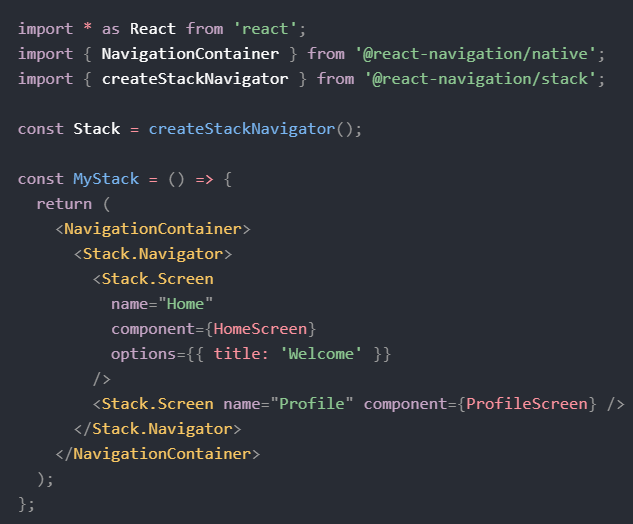
\includegraphics[width=\linewidth]{OpzettenNavigatieReactNative.png}
    \caption{Opzetten navigatie in een React Native applicatie. Bron:
        reactnative.dev/docs/navigation}
    \label{fig:opzettenNavigatieReactNative}
\end{figure}

Vervolgens moet er vastgelegd worden naar welke pagina er genavigeerd moet
worden bij de uitvoering van een bepaald actie, zoals bv de klik op een bepaalde
knop. Om dit mogelijk te maken krijgt elke component die een pagina voorstelt
een attribuut navigation mee. In dit attribuut zitten methodes van de library
die het navigeren tussen de verschillende pagina's mogelijk maakt. De opzet van
een simpele navigatie is te zien in figuur \ref{fig:navigerenReactNative}. 

Zoals eerder vermeld heeft de library zeer veel mogelijkheden en levert het een
navigatie af die native aanvoelt voor de gebruiker. Om dit te bereiken beschikt
React Native Navigation ook over verschillende packages die o.a. tabs en drawer
functionaliteit aanbieden. Dit zijn twee populaire manieren om te navigeren
binnen een applicatie. Door dit aan te bieden in een package moet de
ontwikkelaar niet helemaal zelf deze functionaliteit gaan uitwerken en wordt de
standaard die de gebruiker gewoon is van native applicaties geëvenaard.

\begin{figure}
    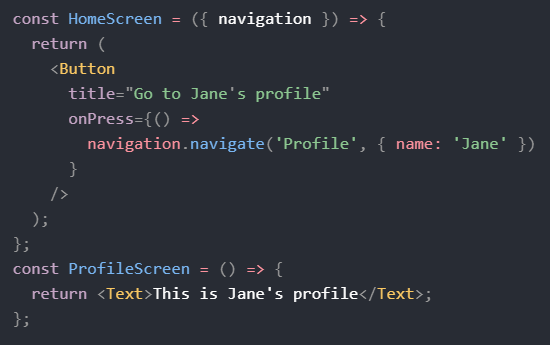
\includegraphics[width=\linewidth]{NavigerenPaginasReactNative.png}
    \caption{Navigeren naar een andere pagina in React Native. Bron:
        reactnative.dev/docs/navigation}
    \label{fig:navigerenReactNative}
\end{figure}

\subsubsection{Flutter}
\label{subsubsec:navigatieFlutter}

Flutter maakt voor de navigatie binnen een applicatie gebruik van de klasse
Navigator. Deze klasse op zich is ook een widget, de bouwstenen van een
applicatie in Flutter. De verschillende pagina's en schermen van een applicatie
worden routes genoemd. Deze routes worden op een stack geplaatst, die de
volgorde van de routes bijhoudt. Er zijn twee verschillende aanpakken van
navigatie binnen Flutter: de ene is gebaseerd op een vaste volgorde waar alle
schermen elkaar opvolgen en de andere laat de ontwikkelaar toe om op aangepaste
wijze te navigeren tussen verschillende pagina's. Beide aanpakken worden in de
volgende paragrafen verder besproken. 

De eerste aanpak laat de gebruiker toe om in een vaste volgorde door de
applicatie te navigeren. Dit is voornamelijk belangrijk als de gebruiker terug
wil gaan naar het vorige scherm. In dit geval is het alleen maar logisch om naar
de vorige route in de stack te gaan. Het is ook meteen de meest eenvoudige vorm
van navigatie. Als de gebruiker naar een andere pagina navigeert wordt deze
bovenaan de stack geplaatst. Indien de gebruiker terug wenst te gaan wordt de
bovenste route terug verwijderd van de stack en komt de gebruiker op de vorige
pagina terecht.

De tweede aanpak is een iets gecompliceerdere aanpak. Deze volgt geen logische
volgorde maar wel de volgorde die vastgelegd is door de ontwikkelaar. De aanpak
berust op een Navigator.pages object. Hieraan kunnen de verschillende pagina's
toegevoegd worden. Vervolgens zal de Navigator dit Navigator.pages object
omzetten in een stack van routes. Indien een nieuwe pagina wordt toegevoegd aan
Navigator.pages dan wordt de stack ook geüpdate. 

\begin{figure}
    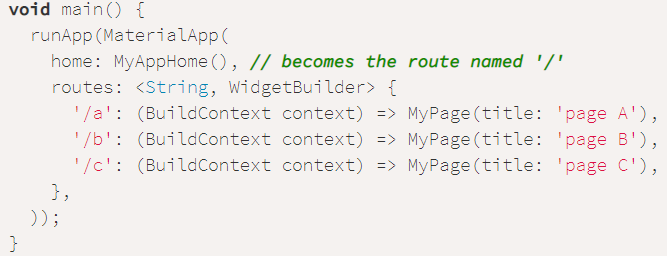
\includegraphics[width=\linewidth]{NamedRoutesFlutter.png}
    \caption{Opzetten navigatie met benoemde routes in Flutter. Bron:
        \textcite{Flutter.dev2020}}
    \label{fig:namedRoutesFlutter}
\end{figure}

\begin{figure}
    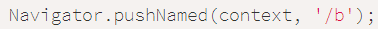
\includegraphics[width=0.5\linewidth]{UseNamedRouteFlutter.png}
    \caption{Benoemde route tonen in Flutter. Bron: \textcite{Flutter.dev2020}}
    \label{fig:useNamedRoutesFlutter}
\end{figure}

Een applicatie kan uit zeer veel verschillende schermen bestaan. Om de navigatie
ertussen overzichtelijk te houden voor de ontwikkelaar beschikt Flutter over een
functie om de routes een naam te geven. Vervolgens kan de pagina aan de hand van
zijn naam getoond worden. In figuur \ref{fig:namedRoutesFlutter} is de definitie
van een map te zien die de naam van een route bevat en de builder die de route
effectief zal tonen op het scherm. In figuur \ref{fig:useNamedRoutesFlutter} is
te zien hoe de route effectief getoond kan worden. Uit de naam van de methode
wordt duidelijk dat ook deze methode gebruik maakt van een stack voor de
navigatie. De nieuwe route wordt bovenop de stack geplaatst.

Beide methodes maken dus gebruik van dezelfde stack en kunnen dus ook door
elkaar gebruikt worden. Dit is een logische aanpak, aangezien een logische
volgorde in een applicatie absoluut noodzakelijk is. Indien een gebruiker terug
wil gaan is het alleen logisch om naar de vorige stap te gaan, ongeacht welke
methode gebruikt werd om naar de huidige pagina te navigeren. 

Verder is het in Flutter mogelijk om een route een waarde te laten terug geven.
Dit is bijvoorbeeld handig indien de gebruiker op oké moet klikken alvorens er
naar het volgende scherm gegaan kan worden. Indien de gebruiker uit dit scherm
gaat door de terug knop van het systeem te gebruiken is de waarde die
teruggegeven wordt null en zal het volgende scherm dus niet getoond worden.

Tot slot geeft de Navigator klasse de ontwikkelaar ook de mogelijkheid om popups
te tonen op het scherm. Dit zijn schermen die niet de volledig oppervlakte van
het scherm in nemen en dus nog een deel van het onderliggende scherm tonen. Het
onderliggende scherm wordt echter geblokkeerd, de gebruiker kan dus enkel binnen
de popup input geven. Deze popups gedragen zich verder als een normale route, de
navigatie naar een popup en er weg van is dus exact hetzelfde.

\subsubsection{Vergelijking navigatie}
\label{subsubsec:vglNavigatie}

Beide frameworks hebben hun eigen techniek om de navigatie aan te pakken. Het
grootste verschil tussen beiden is dat React Native gebruik maakt van een
library, waar Flutter gebruik maakt van een widget. Dit verschil vloeit voort
uit het fundamentele verschil in aanpak tussen beide frameworks. De oorzaak is
dat React Native voor een heel groot deel door de community onderhouden wordt.
Onder andere de library voor navigatie komt voort uit de community en zit dus
niet standaard in React Native, waar dit bij Flutter wel standaard beschikbaar
is.

Voor de volgorde van de navigatie bij te houden maken beide frameworks gebruik
van een stack. Ze zijn dus beide in staat om terug te gaan naar de vorige
pagina. Bij React Native moet elke pagina echter wel steeds benaamd worden om er
naar toe te kunnen navigeren, waar het bij Flutter mogelijk is om op voorhand
een vaste volgorde te definiëren.

In het gevoel voor de gebruiker is er echter geen verschil tussen beide
frameworks. Beide frameworks leveren een navigatie af die overeen komt met de
native navigatie. Verder kan de ontwikkelaar bij beide de overgang tussen de
verschillende pagina's aanpassen om te voldoen aan de uitstraling die de app
wilt geven. 

Er kan besloten worden dat er op het vlak van navigatie geen duidelijk beter
framework is. Er is een verschil tussen de manier waarop de ontwikkelaar de
navigatie implementeerd, maar voor de gebruiker heeft de navigatie met beide
frameworks hetzelfde native gevoel.

\subsection{Toegang native API's}
\label{subsec:toegangNativeAPIs}

Om een applicatie te kunnen afleveren die alle hardware functionaliteiten van
het doelplatform kan gebruiken is het noodzakelijk dat het framework toegang
heeft tot de Native API's van het platform. Ook de manier waarop dit gebeurd is
van belang, hoe efficiënter dit gebeurd, hoe beter de performantie van de
applicatie. Cross-platform frameworks bieden een eigen API aan om met de meest
voorkomende eigenschappen te kunnen werken. Op deze manier hoeven de
ontwikkelaars geen native code of componenten te kennen om een applicatie te
schrijven.

\subsubsection{React Native}
\label{subsubsec:nativeAPIReactNative}

Zoals voor de meeste functionaliteit van het framework rekent React Native op
libraries om specifieke eigenschappen van een platform te kunnen gebruiken. Zo
is er bijvoorbeeld de library React Native Camera. Dit is een library die de
ontwikkelaar toelaat om de camera van een apparaat te gebruiken, ongeacht het
besturingssysteem van het apparaat. Voor de meest voorkomende eigenschappen van
apparaten bestaan er dergelijke libraries. De ontwikkelaar hoeft dus geen native
code te kennen om toch gebruik te kunnen maken van platform specifieke
eigenschappen.

In uitzonderlijke gevallen kan het echter zijn dat de ontwikkelaar een
eigenschap van een bepaald apparaat wil gebruiken waarvoor nog geen library
beschikbaar is. Een applicatie maken die de eigenschappen van een apparaat niet
ten volle gebruikt is uiteraard niet de bedoeling. Om te vermijden dat in dit
geval native ontwikkeling van de applicatie beter zou zijn voorziet React Native
de mogelijkheid om in deze uitzonderlijke gevallen toch native code te gaan
schrijven. Op deze manier kan de ontwikkelaar wel alle eigenschappen gebruiken,
zonder dat het hele project in de native taal geschreven moet worden. De native code wordt omsloten door een native module die ingepast kan worden in de React Native applicatie.

\subsubsection{Flutter}
\label{subsubsec:nativeAPIFlutter}

Flutter maakt voor de toegang tot specifieke eigenschappen van een platform
gebruik van plugins. Zo is er bijvoorbeeld de camera plugin die de ontwikkelaar
toelaat om de camera van een apparaat te gebruiken. De plugin bevat onder meer
methodes om alle beschikbare camera's van een apparaat op te halen (bij een
smartphone bijvoorbeeld de camera aan de voorkant en die aan de achterkant), de
gewenste camera te selecteren en een foto te nemen met deze camera. Voor de
meest voorkomende eigenschappen bestaan er dergelijke plugins. Ook hier hoeft de
ontwikkelaar dus geen native code te kennen om toch specifieke eigenschappen van
een platform te kunnen gebruiken.

Indien de ontwikkelaar eigenschappen van een apparaat wil gebruiken waarvoor nog geen plugin bestaat voorziet Flutter de mogelijkheid om toch native code te gaan schrijven en dit te implementeren in de Flutter applicatie. Flutter voorziet klassen die de communicatie tussen platform-specifieke en Flutter code verzorgen. Deze laten toe om native code te schrijven voor een specifieke toepassing.

\subsubsection{Vergelijking toegang native API's}
\label{subsubsec:vglToegangNativeAPIs}

In de vorige secties werd duidelijk dat beide frameworks de gebruiker in staat stellen om toegang te hebben tot de native API's. Bij beiden zijn er voor de meest voorkomende eigenschappen reeds oplossingen voorzien (bij React Native in de vorm van een library, bij Flutter in de vorm van een plugin). Indien er nog geen standaard oplossing voor bestaat om een bepaalde eigenschap te gebruiken laten beide frameworks de ontwikkelaar toe om alsnog native code te gaan schrijven. De ontwikkelaar heeft dus steeds gegarandeerd toegang tot alle eigenschappen van een apparaat. Kennis van de native code is wel nodig in deze omstandigheden bij beide frameworks.


